\documentclass[../main.tex]{subfiles}

\begin{document}
	\section{Resultate}
	
	\subsection{Frontend}
	
	Als Frontend haben wir 3 Menüpunkte ausgewählt, welche die Hauptfaktoren unserer Schnittstelle aufzeigen. \\
	Der erste Punkt ist die Übersicht. Hier werden die aktuellen Systeme mit Tanks und die Hauptsensorendaten aufgeführt. \\
	Für alle Sensorendaten gibt es einen Editierbutton, mit welchem die Daten geändert werden können.\\
	Unterhalb jedes Systems gibt es die Details Option. Über diesen gelangt man zu den detaillierten Infos jedes Tanks des oben genannten Systems in der unteren Abbildung \gls{angular} Frontend. \\ \\
	Das tabellarische Layout ist an das Design des \gls{sc1000} angelehnt, damit mit einer gewohnten Umgebung weitergearbeitet werden kann. 
	\begin{figure}[H]
		\centering
		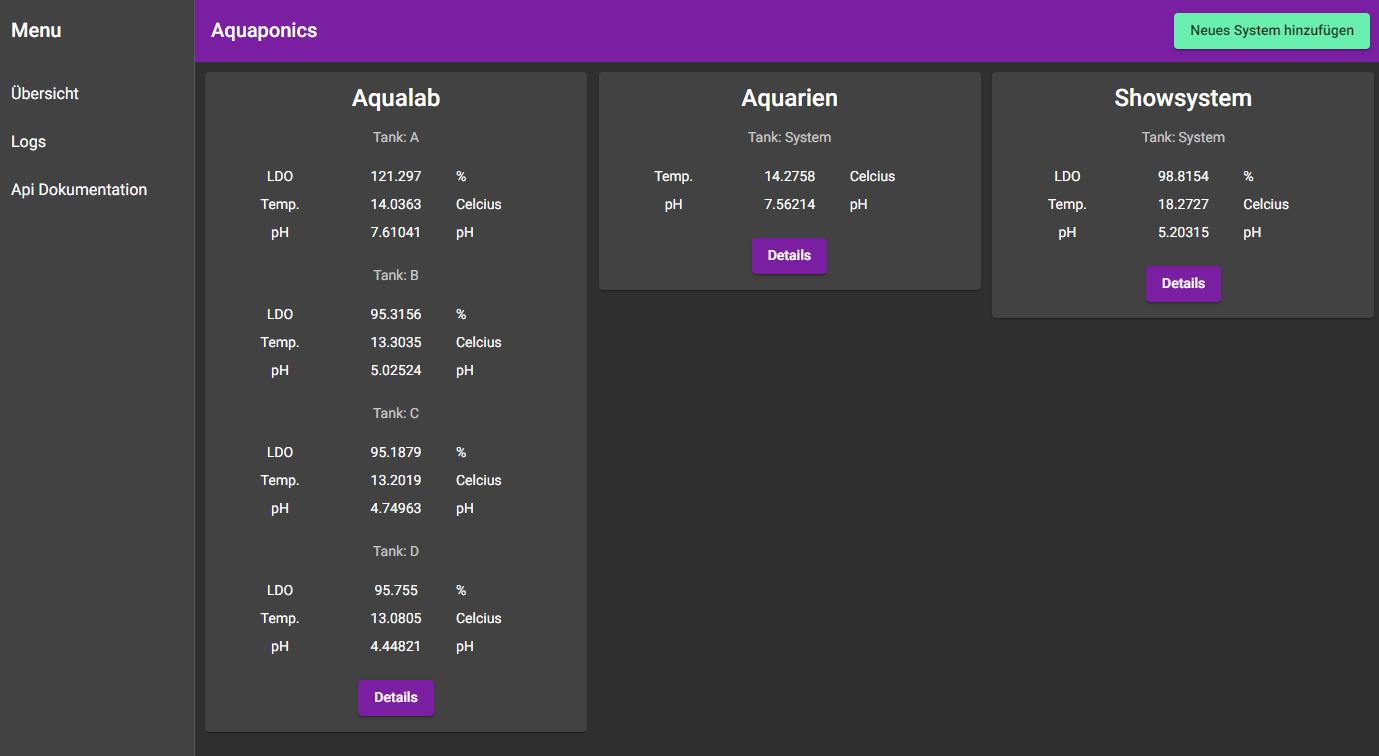
\includegraphics[scale=0.4]{Frontend_Dashboard}
		\caption{Übersicht}
		\label{fig:Frontend_Dashboard}
	\end{figure}
	\par
	\noindent
	Der zweite Punkt ist Logs. Hier sind alle Daten über einen älteren Zeitraum archiviert worden. Die Daten sind wichtig um zu vergleichen, wie sich Veränderungen über eine längere Zeit gebildet haben. Die Logdaten sind eins zu eins aus der Datenbank geladen und werden dort immer aktualisiert. Hier sind auch Sensorennummer und Zeitstempel enthalten damit keine Verwirrung auftritt.
	
	\begin{figure}[H]
		\centering
		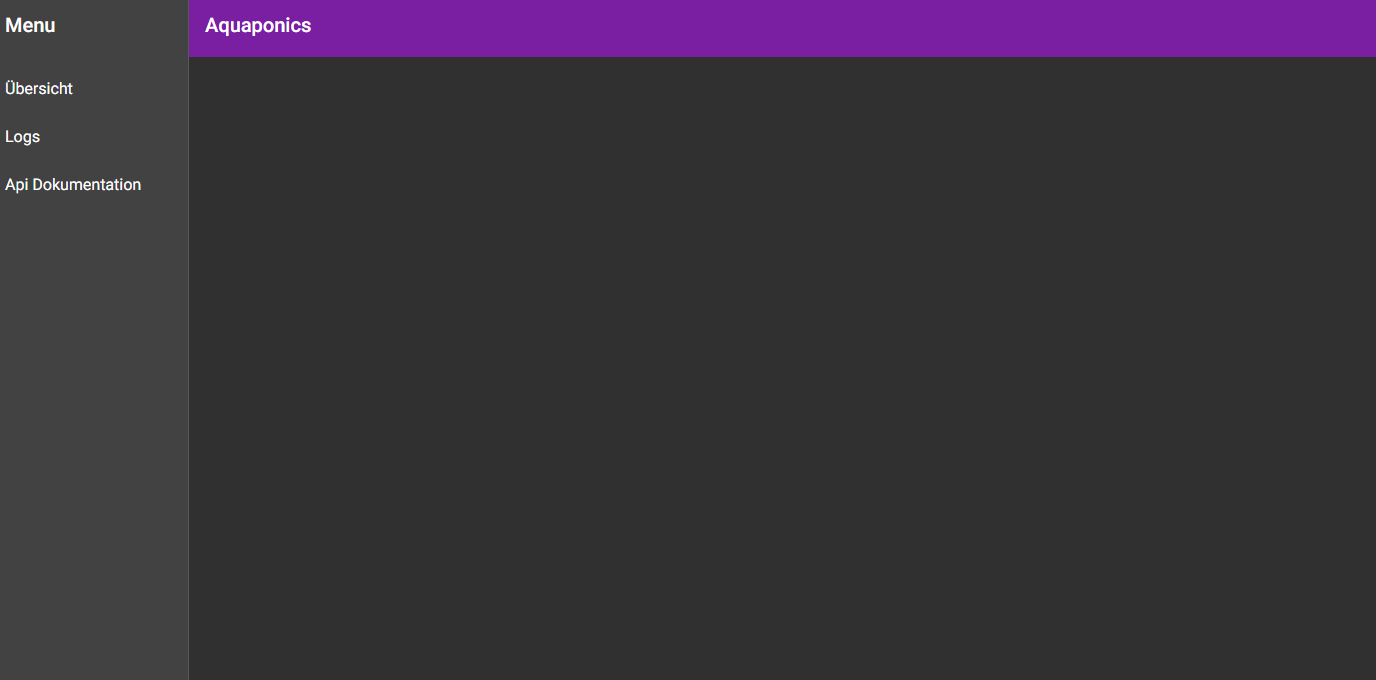
\includegraphics[scale=0.4]{Frontend_Logs}
		\caption{Logs}
		\label{fig:Frontend_Logs}
	\end{figure}
	\par
	\noindent
	Als letzter Menüpunkt wird noch auf die \gls{api} Dokumentation verwiesen, welche sich auf die Swagger UI bezieht. Dort sieht man alle Eigenschaften und andere Wissenswerte Details über die Schnittstelle für zukünftige Entwicklungen.\par 
	\begin{figure}[H]
		\centering
		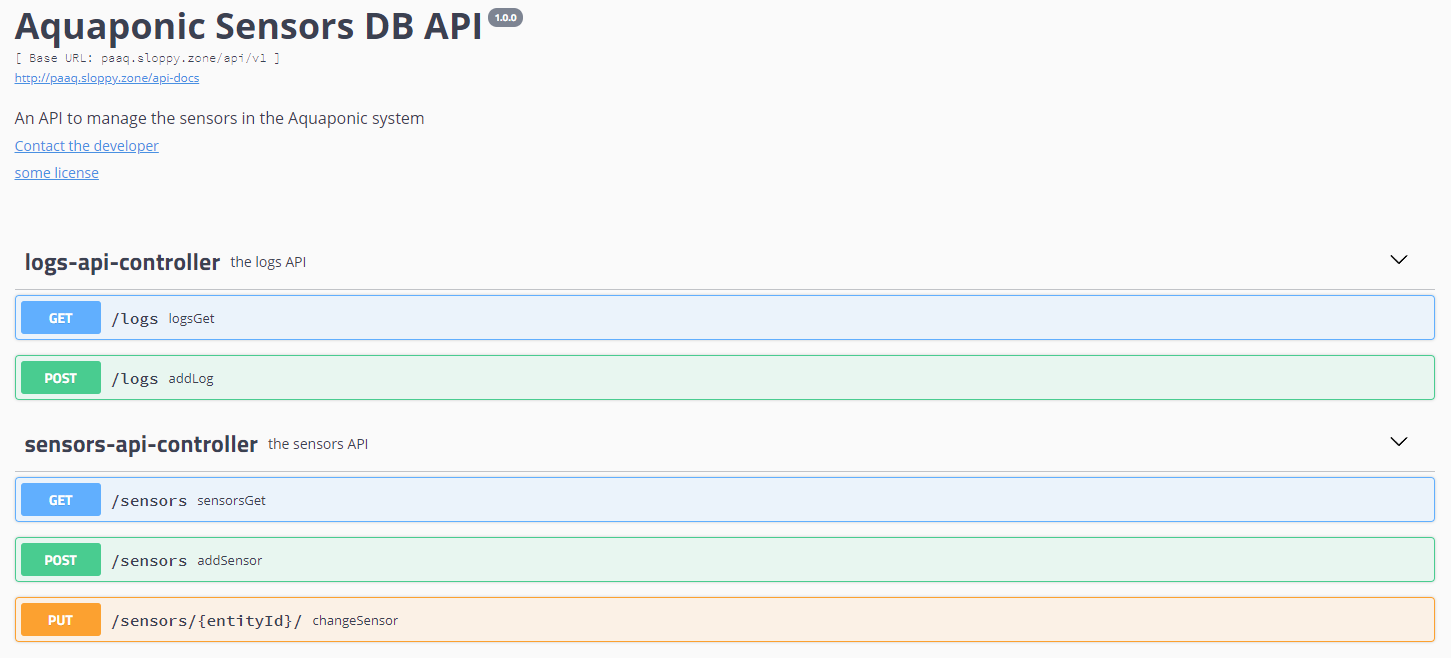
\includegraphics[scale=0.4]{../images/API_Documentation}
		\caption{API Dokumentation}
		\label{fig:API_Documentation}
	\end{figure}
	\noindent
	Wie auf der Abbildung ersichtlich ist, werden verschiedene \gls{api} Aufrufe über das Aufrufen des Dashboards oder das Klicken auf den Editierbutton in den Sensorendaten gesteuert. 
	\\
	Somit wird das Arbeiten mit den Sensorendaten um ein Vielfaches erleichtert.
	
	%------------------------------------------------------------------
	
	\subsection{Backend}
	Unser Backend besteht aus einem Spring Boot Server und einer MySQL-Datenbank. Zudem besteht ist es Möglich, den Spring Boot Server in einem Docker Image zu verwenden.
	
	\subsubsection{Spring Boot Server}
	Spring Boot ermöglichte uns einen schnellen Start, indem es viele der \gls{boilerplate} lastigen Themen übernimmt und direkt zur Verfügung stellt. Die Anbindung der Datenbank, das Handhaben von Websockets und die Abhandlung von klassischen Fehlerquellen wie nicht gefundenen Resourcen seitens des Servers wurden somit direkt von Spring Boot gehandhabt. Somit konnten wir uns auf die Themen fokussieren, die unseren Server von anderen Servern unterscheiden wird, sprich wie er die Schnittstelle zur Verfügung stellen wird.
	
	Basierend auf der \gls{interfacefirst} Herangehensweise, konnten wir per OpenAPI-Generator einen Teil des Servers automatisch generieren. Datenodelle, API und Controller liessen sich in einer ersten Form auf diese Weise rasch erzeugen. Die Verbindung der generierten Komponenten zur Datenbank wurde von uns manuell programmiert.
	
	\subsubsection{Datenbank}
	Als Datenbank verwenden wir eine MySQL-Datenbank, die mithilfe eines offiziellen MySQL Docker Image in einem Container läuft. Zusätzlich zum Datenbank-Container ist auch noch ein \gls{phpmyadmin} Container in Betrieb, der es dem Team der ZHAW Wädenswil ermöglicht, die Daten wie zuvor zu begutachten oder zu editieren.
	
	Als Datenbank-Schema haben wir das Schema der bisher vom Team der ZHAW Wädenswil gebrauchten Datenbank verwendet. Dies hauptsächlich deswegen, weil der Wunsch geäussert wurde, die alten Daten beizubehalten und auch den neuen Einarbeitungsaufwand klein zu halten.
	
	\subsubsection{Docker}
	Die zwei erwähnten Systeme laufen in drei \gls{docker} \gls{container}n da \gls{mysql} und \gls{phpmyadmin} in einzelnen \gls{container}n laufen. Alle drei \gls{container} sind in einem Containernetzwerk miteinander verbunden und können untereinander kommunizieren ohne dass der Verkehr nach aussen gelangt. Nur der \gls{springboot} \gls{container} und der \gls{phpmyadmin} \gls{container} ist von aussen erreichbar, da im Containernetzwerk ein \gls{portforwarding} für diese zwei \gls{container} eingerichtet wurden.
	
	\subsection{OpenAPI Generator und Swagger}
	
\end{document}